\documentclass{standalone}
\usepackage{tikz}
\usepackage{ctex,siunitx}
\usepackage{tkz-euclide}
\usepackage{amsmath}
\usetikzlibrary{patterns, calc}
\usetikzlibrary {decorations.pathmorphing, decorations.pathreplacing, decorations.shapes,}
\begin{document}
\small
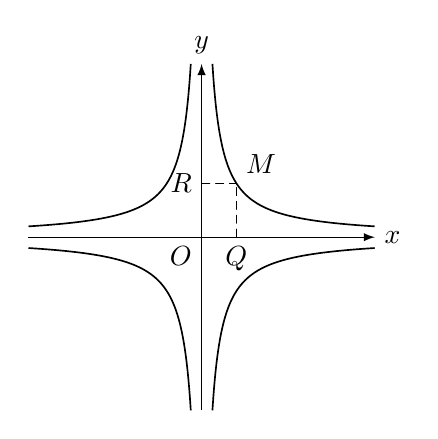
\begin{tikzpicture}[>=latex,scale=0.55,samples=200]
  % \useasboundingbox(0,-0.2)rectangle(3,0.5);
  \draw[thin,->](-4,0)--(4,0)node[right]{$x$};
  \draw[thin,->](0,-4)--(0,4)node[above]{$y$};
  \draw [semithick,domain=0.25:4]  plot (\x,{1/\x});
  \draw [semithick,domain=0.25:4]  plot (\x,{-1/\x});
  \draw [semithick,domain=-0.25:-4]  plot (\x,{1/\x});
  \draw [semithick,domain=-0.25:-4]  plot (\x,{-1/\x});
  \tkzDefPoints{0/1.25/R,0.8/0/Q,0.8/1.25/M,0/0/O}
  \tkzDrawSegments[densely dashed](R,M Q,M)
  \tkzLabelPoints[left](R)
  \tkzLabelPoints[above right](M)
  \tkzLabelPoints(Q)
  \tkzLabelPoints[below left](O)
\end{tikzpicture}
\end{document}